\documentclass[tikz,border=10pt]{standalone}
\usetikzlibrary{intersections,calc}

\begin{document}
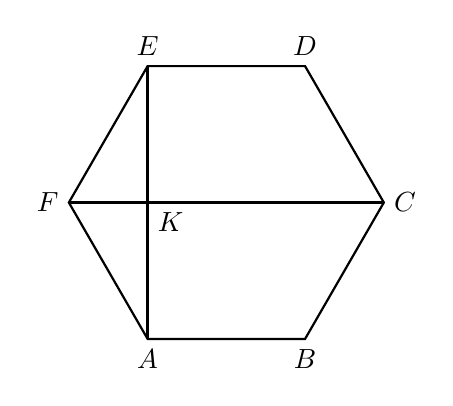
\begin{tikzpicture}[scale=2, thick]
    % 1. 定义正六边形顶点坐标 (半径为 1)
    % C 为右侧顶点，按逆时针旋转依次定义
    \coordinate (C) at (0:1);
    \coordinate (D) at (60:1);
    \coordinate (E) at (120:1);
    \coordinate (F) at (180:1);
    \coordinate (A) at (240:1);
    \coordinate (B) at (300:1);

    % 2. 绘制正六边形边界
    \draw (A) -- (B) -- (C) -- (D) -- (E) -- (F) -- cycle;

    % 3. 绘制辅助线 FC 和 AE
    \draw[name path=FC] (F) -- (C);
    \draw[name path=AE] (A) -- (E);

    % 4. 计算交点 K
    \path [name intersections={of=FC and AE, by={K}}];

    % 5. 标注顶点和点 K
    \node[below] at (A) {$A$};
    \node[below] at (B) {$B$};
    \node[right] at (C) {$C$};
    \node[above] at (D) {$D$};
    \node[above] at (E) {$E$};
    \node[left] at (F) {$F$};
    \node[below right] at (K) {$K$};

    % 可选：标记交点 K 的位置（若需要小圆点）
    \fill (K) circle;

\end{tikzpicture}
\end{document}